%-----------------------------------------------------------------------------%
\chapter{\babLima}
%-----------------------------------------------------------------------------%
Pada bagian ini dijelaskan mengenai pengembangan \f{high-fidelity prototype} dengan menggunakan aplikasi berbasis \f{web} yang bernama InvisionApp. \f{Prototype} yang diolah pada InvisionApp menghasilkan sebuah \f{clickable prototype}.
%-----------------------------------------------------------------------------%
\section{Perancangan Strategi Perbaikan}
Sebelum memasuki tahap pembuatan tampilan antarmuka, penulis terlebih dahulu membuat perancangan strategi berdasar dari masukkan responden dan hasil analisis evaluasi \f{usability e-government}. Pada hasil analisis data diketahui bahwa \f{website} DJP Indonesia memiliki tingkat efisiensi yang kurang dikarenakan tingkat \f{cognitive effort}-nya rendah, sehingga membutuhkan usaha lebih bagi pengguna awam untuk mempelajari \f{website} DJP Indonesia ini. Mengacu pada \f{usability heuristic} dan \f{g-quality} maka dibuat strategi pengembangan perbaikan tampilan dari hasil rekomendasi seperti pada tabel \ref{tab:strategi}.

\begin{center}
	\begin{longtable}{|p{0.5cm}|p{4.5cm}|p{6.5cm}|}
		\caption{Implementasi \f{usability e-government} untuk implementasi tampilan antarmuka}
		\label{tab:strategi}\\
		\hline
		\textbf{No.} & \textbf{Indikator} & \textbf{Implementasi} \\ \hline \endhead
		1 & \f{Visibility of system status} & Pada setiap halaman terdapat keterangan mengenai posisi penjelajahan \f{website} dan sistem \f{website} akan memberitahukan bila pengguna melakukan tindakan diluar kendali sistem. \\ \hline
		2 & \f{Match between system and the real world} & Bahasa yang dipakai oleh sistem \f{website} menggunakan bahasa Indonesia yang ramah terhadap pengguna awam. \\ \hline
		3 & \f{User control and freedom} & Pengguna \f{website} akan lebih leluasa mengakses menu yang menuju ke halaman lain dengan \f{dropdown} menu yang \f{intuitive} mengikuti pengguna. \\ \hline
		4 & \f{Consistency and standards} & Setiap halaman \f{website} memakai skema desain yang sama. \\ \hline
		5 & \f{Error prevention} & Mengingatkan pengguna ketika akan meninggalkan \f{website} dari aktivitas yang sedang dilakukannya. \\ \hline
		6 & \f{Recognition rather than recall} & Alur penggunaan menu dan struktur sistem \f{website} yang mudah membuat pengguna mengingat apa yang lebih dibutuhkannya. \\ \hline
		7 & \f{Flexibility and efficiency of use }& Sistem \f{website} menyimpan \f{cache} dan \f{cookies} pengguna sehingga sistem akan mengenali pengguna dan menggunakan ulang datanya. \\ \hline
		8 & \f{Aesthetics and minimalist design} & Skema tampilan antarmuka yang digunakan adalah desain \f{flat}. Dengan ciri khas tampilan sederhana, kombinasi warna dan layout meminimalisir elemen desain yang tidak diperlukan. \\ \hline
		9 & \f{Help users recognize, diagnose, and recover from errors} & Sistem \f{website} dapat membantu pengguna bila mengalami masalah dengan memberi petunjuk untuk keluar dari halaman tersebut. \\ \hline
		10 & \f{Help and documentation} & Memperbaiki bentuk FAQ dan tutorial menjadi bentuk yang lebih kompak dan teratur sehingga informasi lebih komplit. \\ \hline
		11 & \f{Accessibility} & Membuat tampilan yang sederhana sehingga semua orang dapat memahami dan menggunakan \f{website}. \\ \hline
		12 & \f{Interoperability} & Membuat akses informasi kepada \f{website e-government} lainnya sehingga pertukaran informasi menjadi lebih mudah. \\ \hline
		13 & \f{Security and privacy} & Penambahan kode keamanan pada halaman \f{login} di aplikasi \f{e-filling}. \\ \hline
		14 & \f{Information truth and precision} & Keterangan mengenai informasi dibagi kedalam halaman yang didesain menampung informasi rilis resmi dari \f{website}. \\ \hline
		15 & \f{Service Agility} & Desain transisi halaman dibuat sederhana sehingga meningkatkan kecepatan akses, selain itu dibuat kotak kontak \f{website} yang memberikan pelayanan cepat tanggap. \\ \hline
		16 & \f{Transpareny} & Desain dibuat dengan memperhatikan keterbukaan informasi publik. \\ \hline
	\end{longtable}
\end{center}
%-----------------------------------------------------------------------------%
\section{\f{Clickable-Prototype}}
Pada tahap pengembangan \f{prototype} penulis menggunakan aplikasi berbasis \f{web} \textbf{InvisionApp.com} yang telah dijelaskan pada subbab \ref{subsec:invisionapp}. Sebelum melakukan pembuatan \f{prototype}, penulis mendesain terlebih dahulu tampilan yang direkomendasikan untuk diperbaiki pada \f{prototype} berdasar dari \f{open-ended question usability testing} dengan responden, proses desain dijalankan menggunakan strategi yang telah dibahas pada subbab sebelumnya. Hasil desain kemudian diunggah pada website invisionapp.com untuk dikembangkan menjadi \f{clickable prototype}. Berikut merupakan \f{clicakble prototype} berdasarkan rekomendasi perbaikan:
\begin{enumerate}
	\item Halaman Beranda \\
	Halaman ini didesain berdasarkan tabel rekomendasi perbaikan. Desain dan pengembangannya disesuaikan dengan strategi desain sehingga memenuhi aspek yang dijadikan komponen dalam pengujian \f{usability testing}. Halaman didesain secara sederhana sehingga memenuhi kriteria pada komponen \f{usability heuristic}. Penyederhanaan menu dilakukan pada halaman beranda dengan maksud agar pengguna lebih mudah dalam pengoperasian \f{website}.
	\begin{figure}
		\centering
		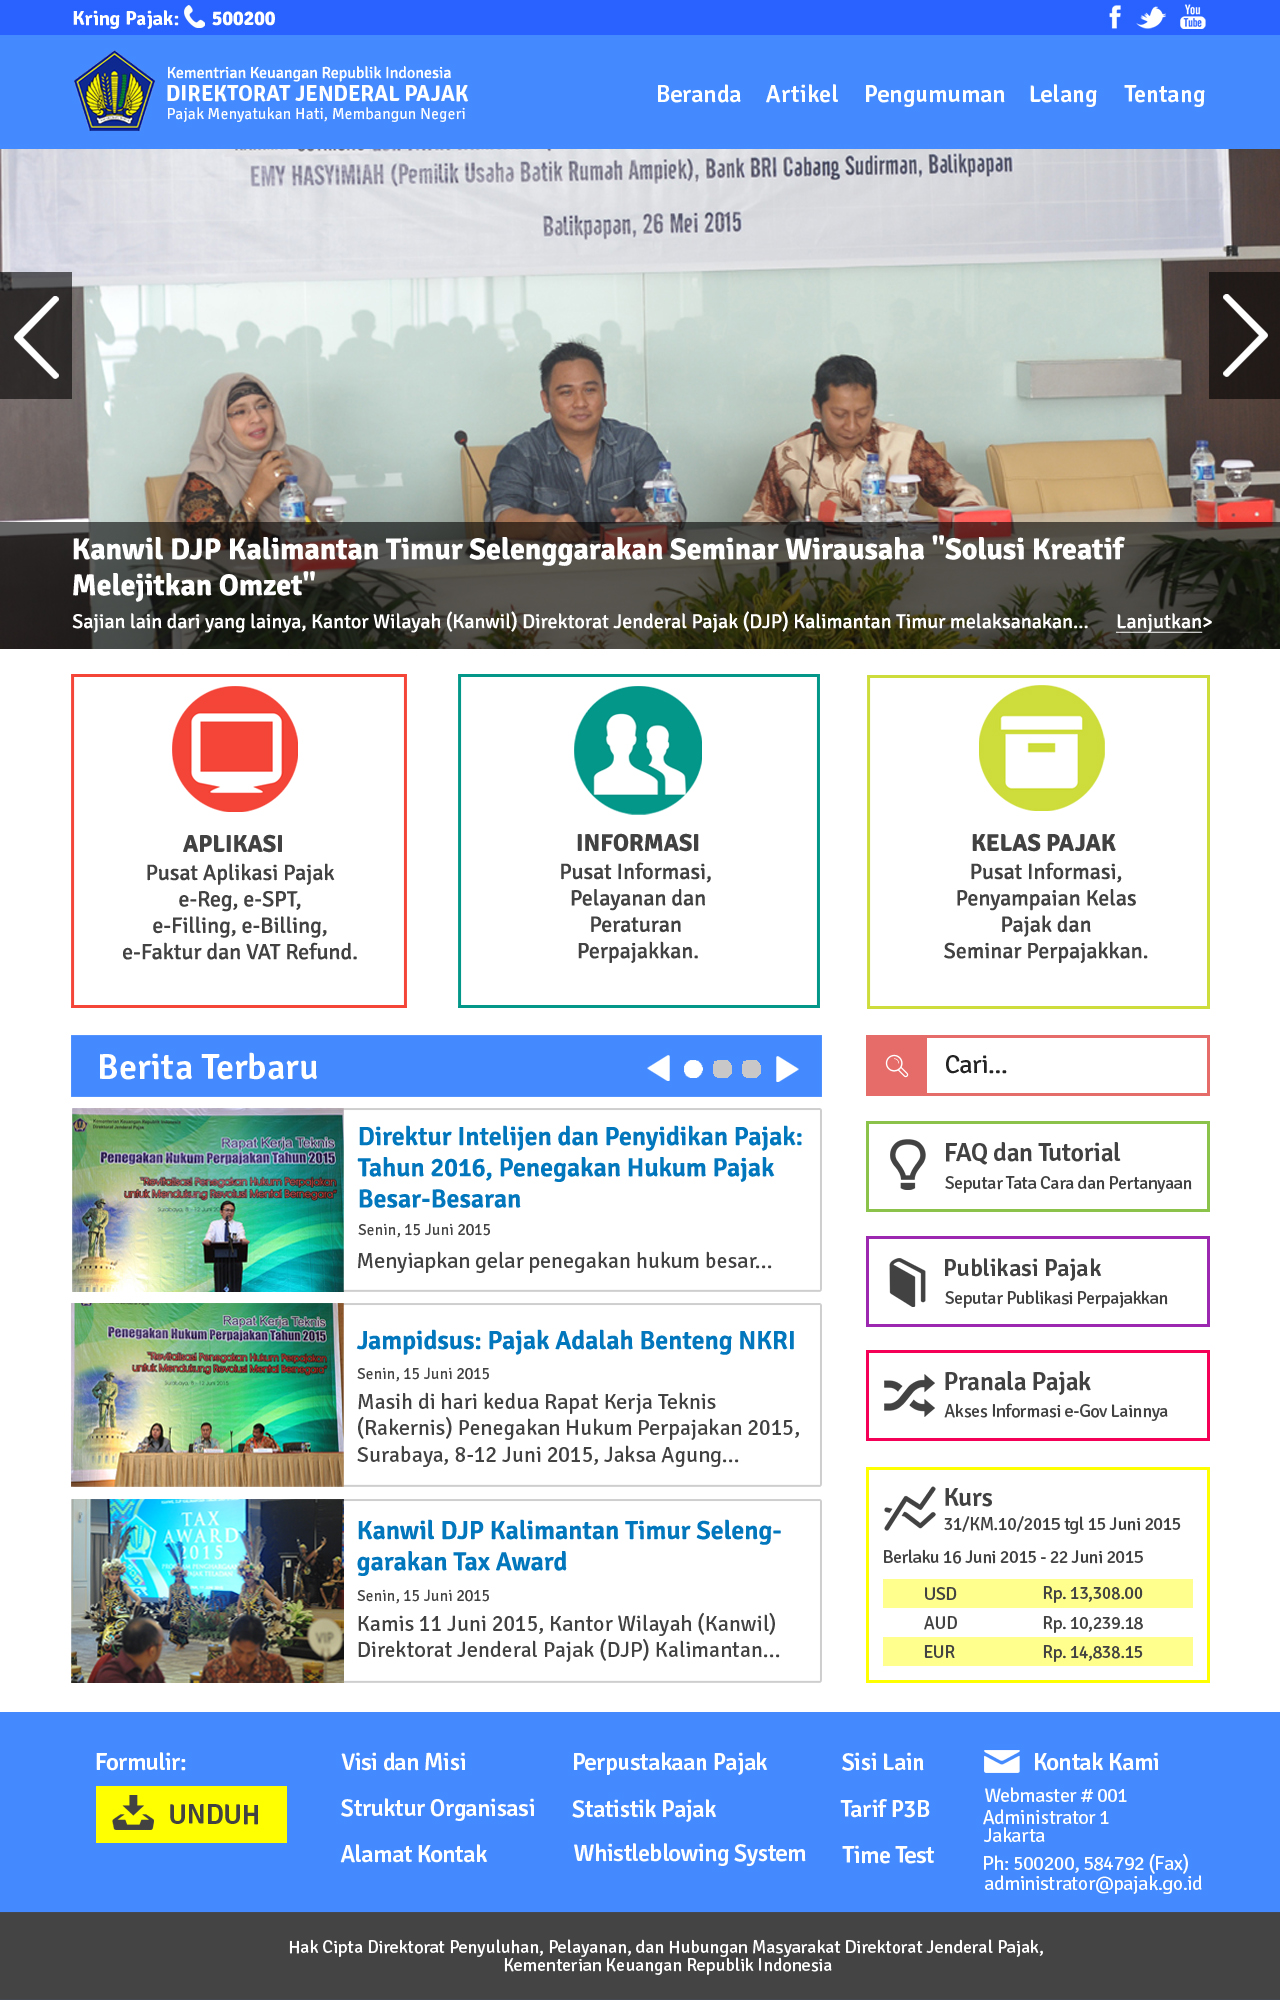
\includegraphics[width=\textwidth]
		{pics/beranda.jpg}
		\caption{\f{Clickable prototype} dari halaman beranda.}
		\label{fig:beranda}
	\end{figure}
	\item Halaman Artikel \\
	Halaman artikel dalam pengembangannya dibagi menjadi 3 bagian. Hal ini dikarenakan artikel memiliki kategori pengelompokkan, sehingga terdapat 3 buah desain yang diperlukan dalam pengembangan \f{clickable prototype}. Desain \f{clickable prototype} pada gambar \ref{fig:artikel} merupakan desain yang diperuntukkan melihat secara detail sebuah artikel, desain ini juga digunakan sebagai dasar semua konten tulisan yang digunakan pada \f{website}.
		\begin{figure}
			\centering
			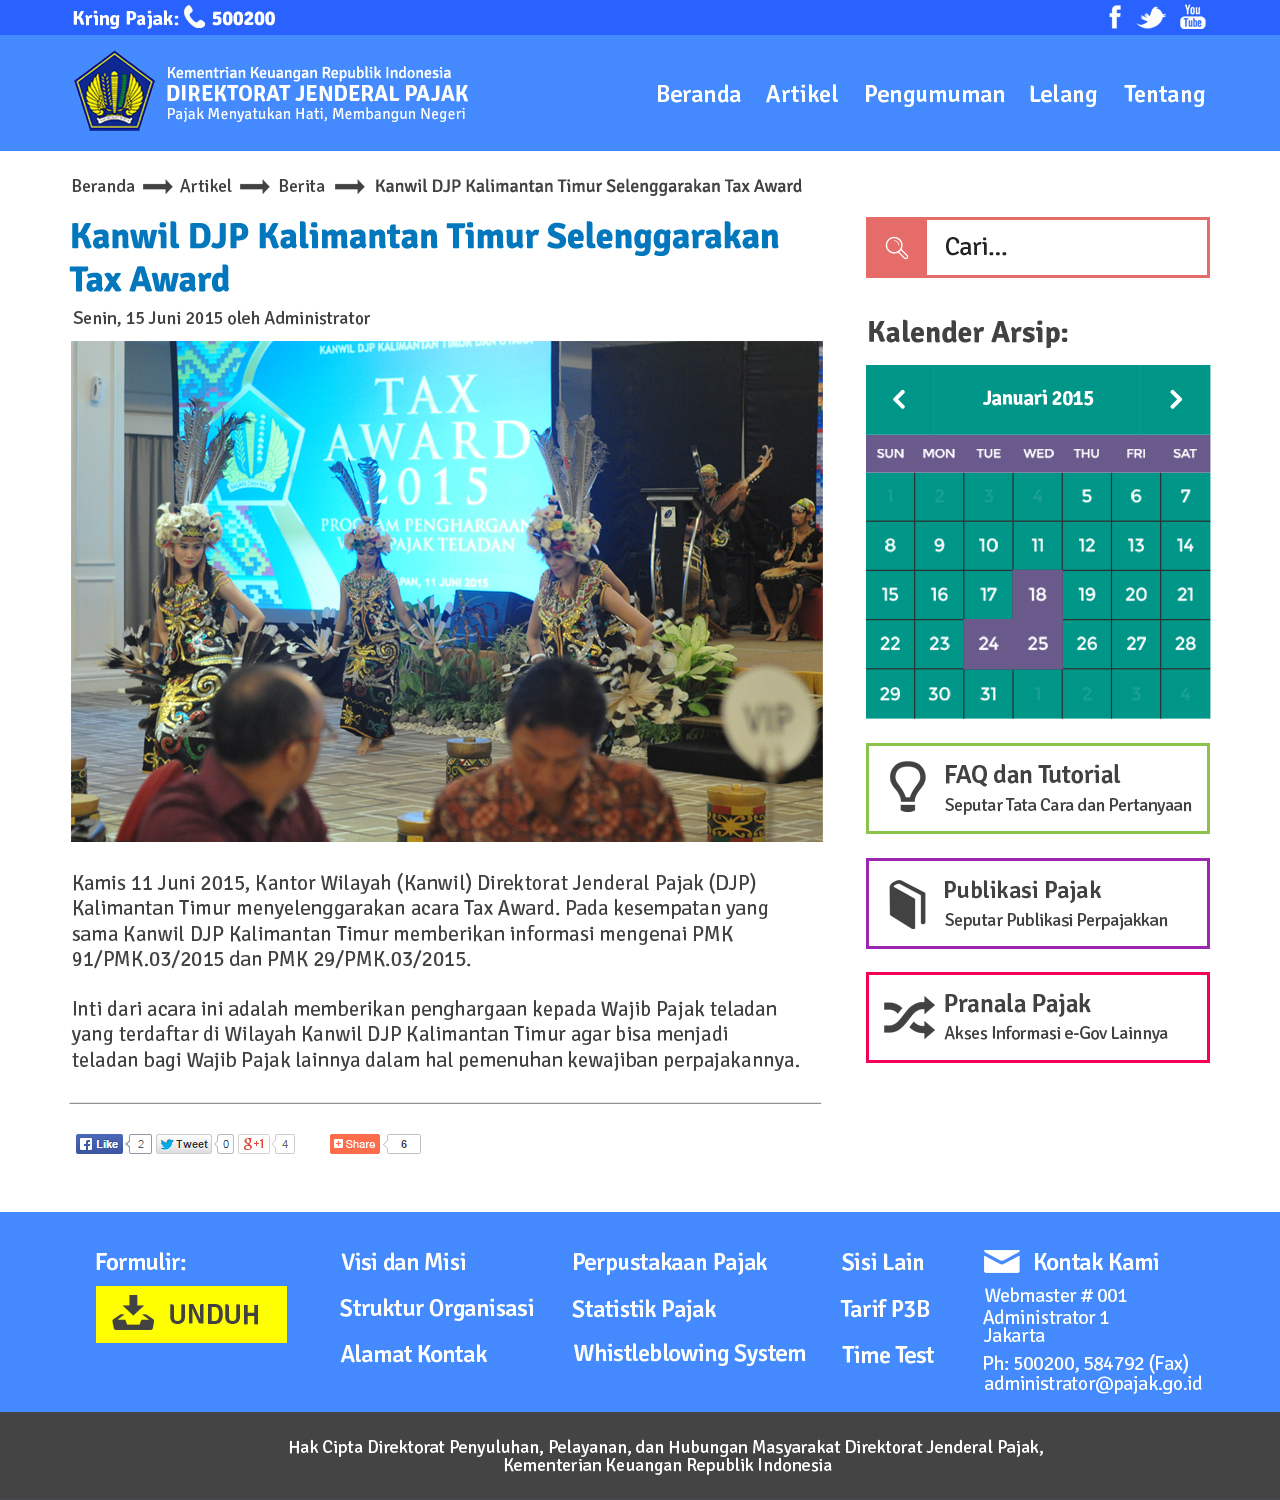
\includegraphics[width=\textwidth]
			{pics/Artikel.jpg}
			\caption{\f{Clickable prototype} dari halaman detail artikel.}
			\label{fig:artikel}
		\end{figure}
	\pagebreak
	Selanjutnya terdapat desain dimana sebuah halaman artikel memuat semua kategori artikel yang dimiliki. Gambar \ref{fig:artikelgrup} menunjukkan halaman dengan semua artikel kategori yang diringkas didalamnya. Pembagian kategori ini dimaksudkan agar pengguna lebih mudah mengidentifikasi jenis dari suatu artikel.
		\begin{figure}
			\centering
			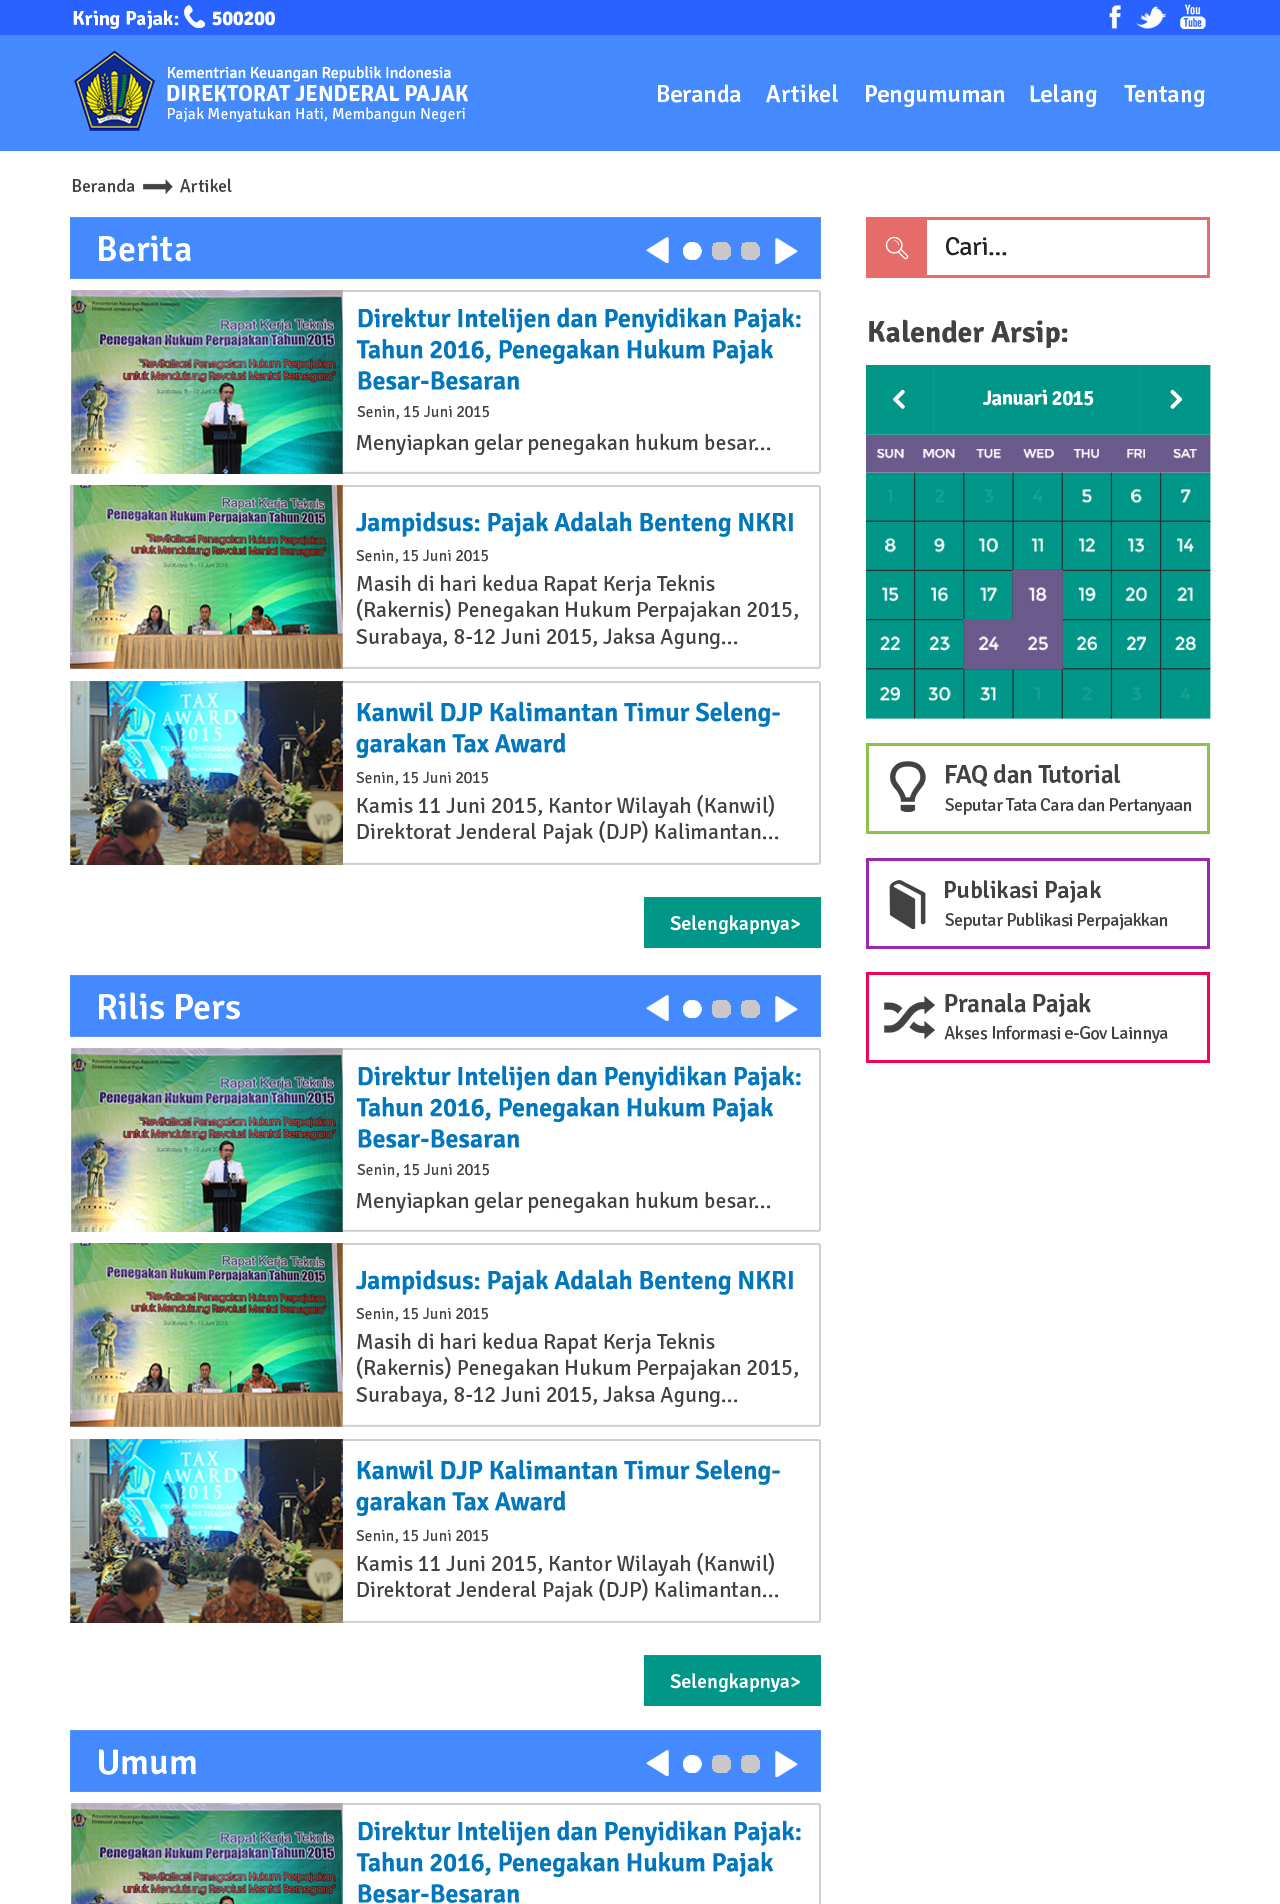
\includegraphics[width=\textwidth,height=23cm]
			{pics/Artikelgrup.jpg}
			\caption{\f{Clickable prototype} dari halaman Artikel dengan mengelempokkan kategori.}
			\label{fig:artikelgrup}
		\end{figure}
	Pada gambar \ref{fig:artikelsatugrup} menunjukkan bahwa halaman ini menampilkan sebuah kategori artikel secara utuh. Pengguna dapat mengeksplorasi lebih jauh artikel suatu kategori secara lebih mendalam pada halaman ini.
		\begin{figure}
			\centering
			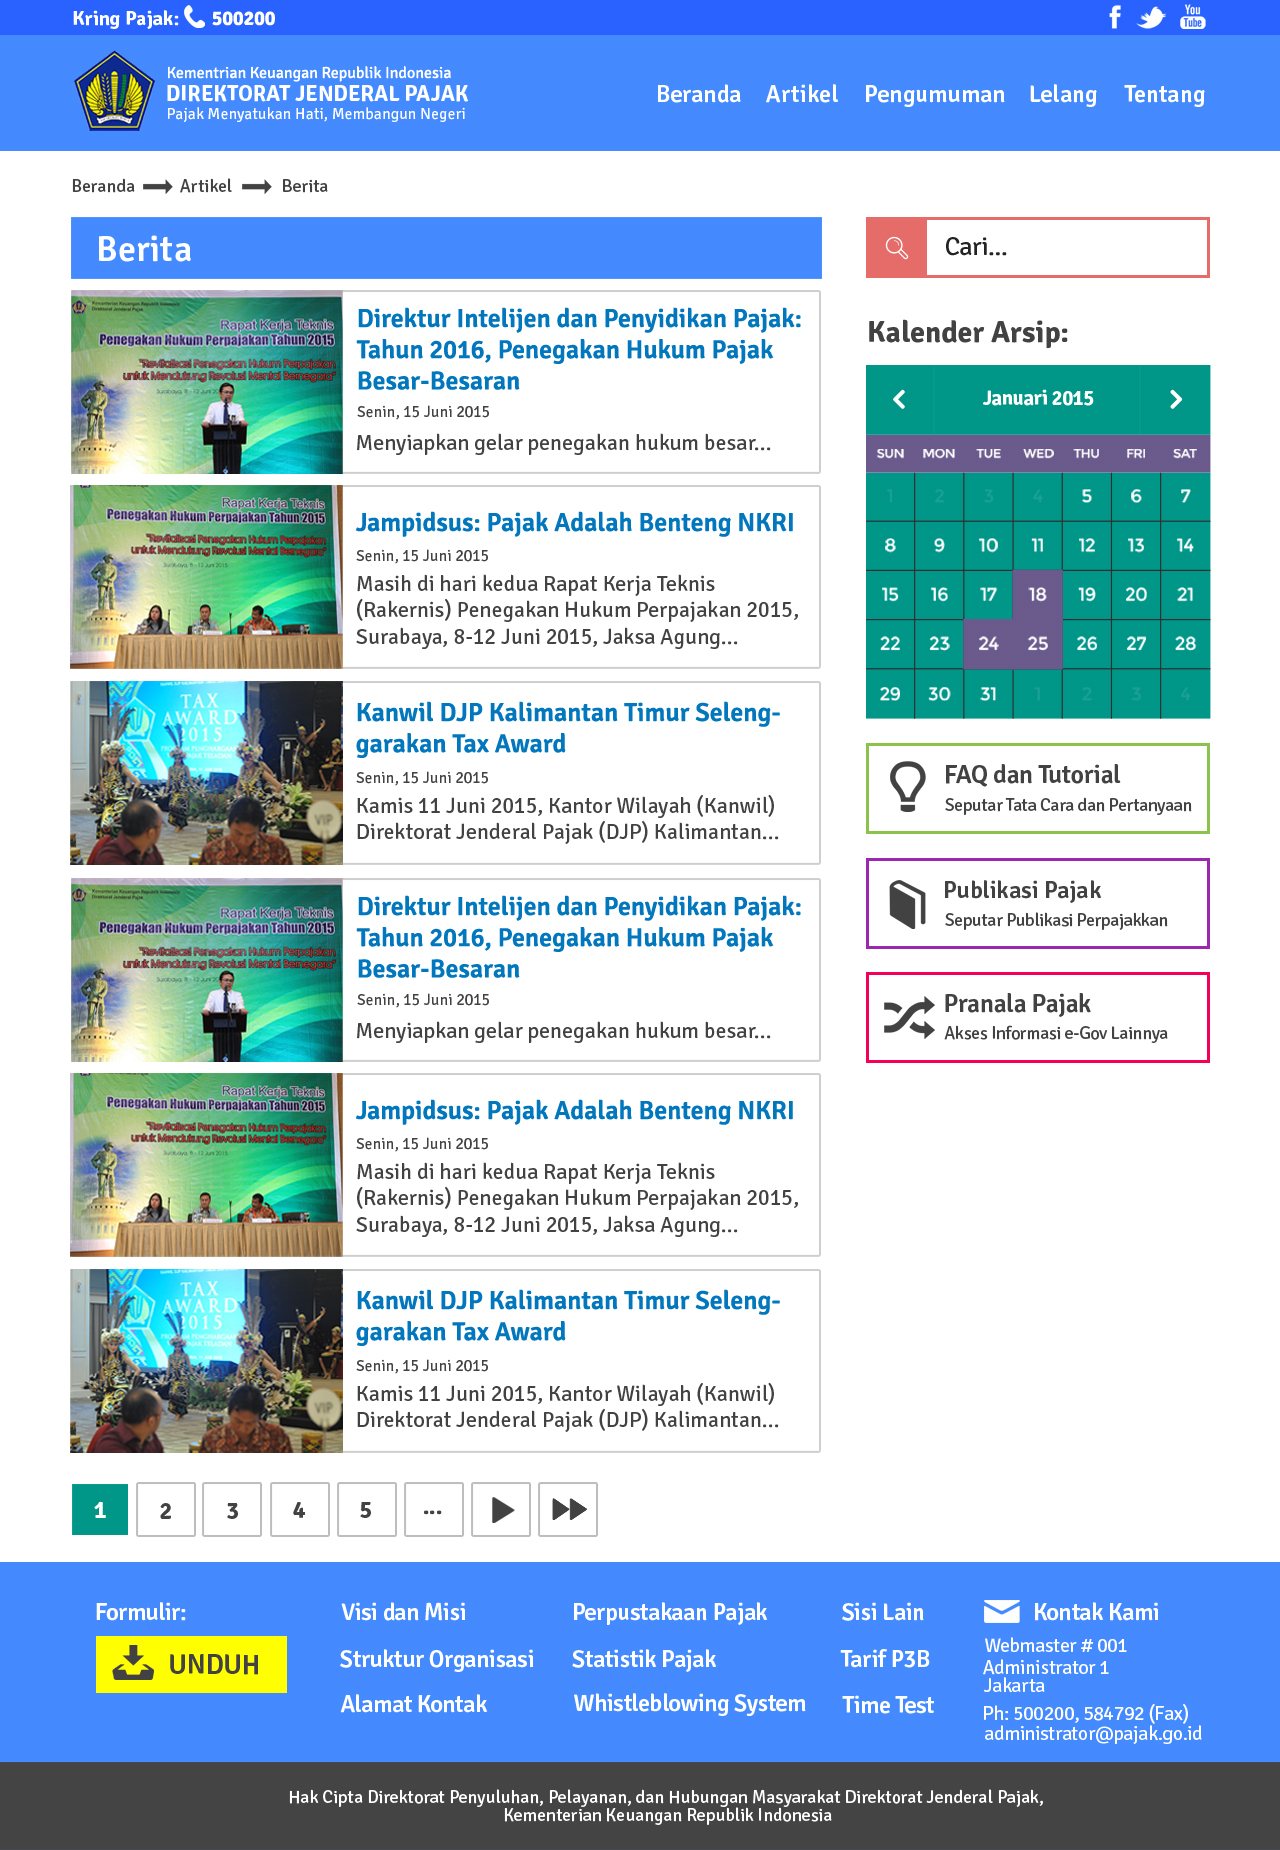
\includegraphics[width=\textwidth]
			{pics/artikelsatugrup.jpg}
			\caption{\f{Clickable prototype} dari halaman artikel hasil pemilihan salah satu dari kategori.}
			\label{fig:artikelsatugrup}
		\end{figure}
	\item Halaman Aplikasi \\
	Halaman aplikasi didesain agar pengguna lebih leluasa dan mudah dalam mengakses aplikasi perpajakkan. Gambar \ref{fig:aplikasi} menunjukkan susunan aplikasi yang dipisah agar lebih jelas maksud dan tujuan penggunaannya.
		\begin{figure}
			\centering
			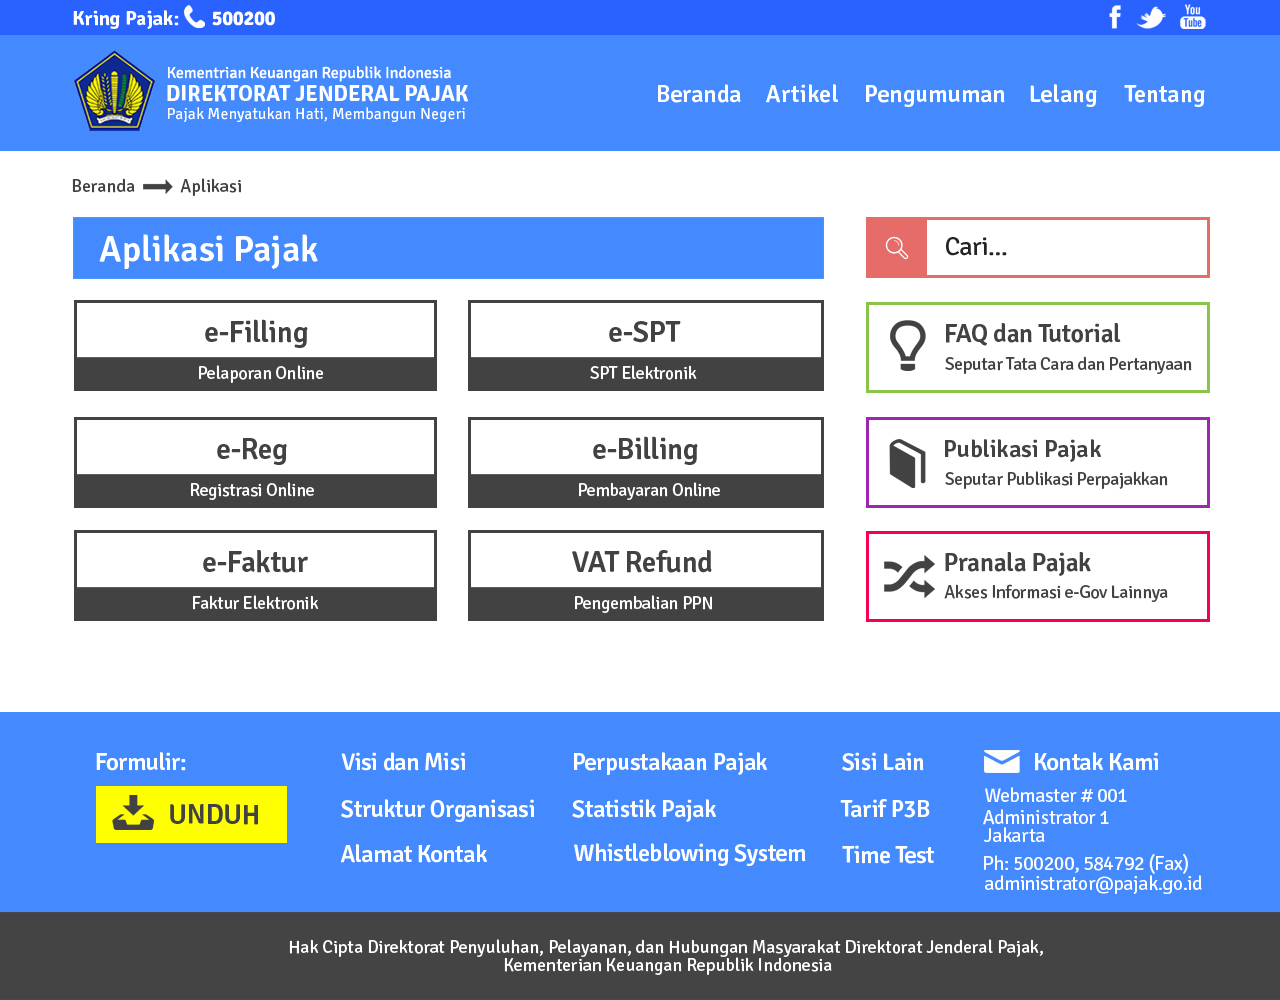
\includegraphics[width=\textwidth]
			{pics/Aplikasi.jpg}
			\caption{\f{Clickable prototype} dari halaman aplikasi.}
			\label{fig:aplikasi}
		\end{figure}
	\item Halaman Pengumuman \\
	Halaman pengumuman didesain sesuai dengan dasar dari halaman artikel. Halaman \f{clickable prototype} pengumuman mengelompokkan jenis pengumuman yang dimiliki oleh \f{website} DJP Indonesia seperti yang terlihat pada gambar \ref{fig:pengumuman}.
		\begin{figure}
			\centering
			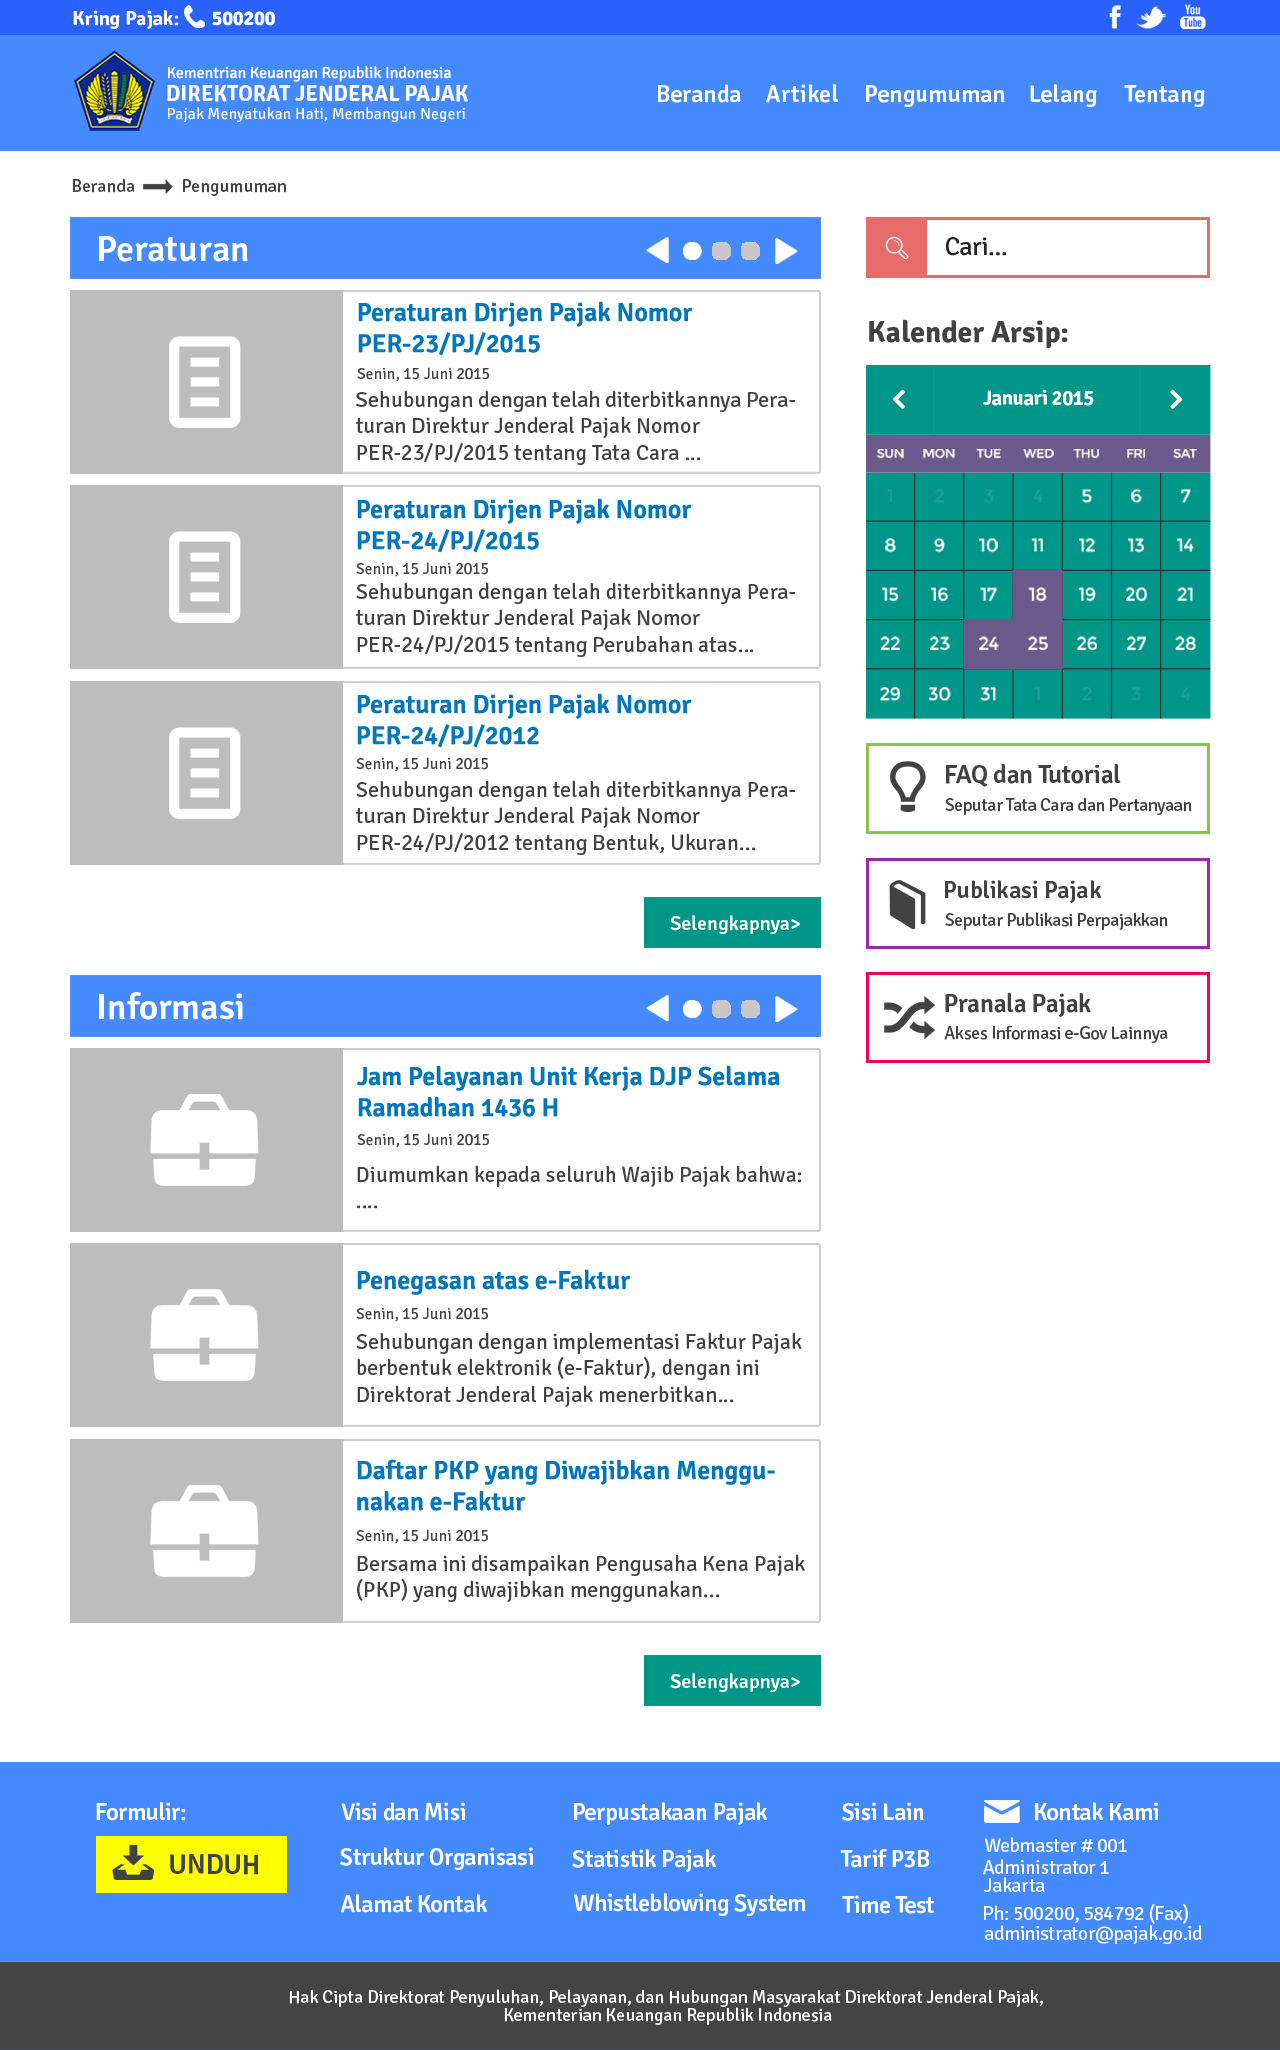
\includegraphics[width=\textwidth]
			{pics/pengumuman.jpg}
			\caption{\f{Clickable prototype} dari halaman pengumuman.}
			\label{fig:pengumuman}
		\end{figure}
	\item Halaman Pesan \f{Error} \\
	Halaman ini didesain untuk memberi tahu pengguna apabila mengakses suatu hal yang tidak diinginkan dan menjurus ke kesalahan sistem tanpa pemberitahuan. Gambar \ref{fig:error} menunjukkan bahwa pengguna telah mengakses sesuatu yang tidak ada pada sistem.
		\begin{figure}
			\centering
			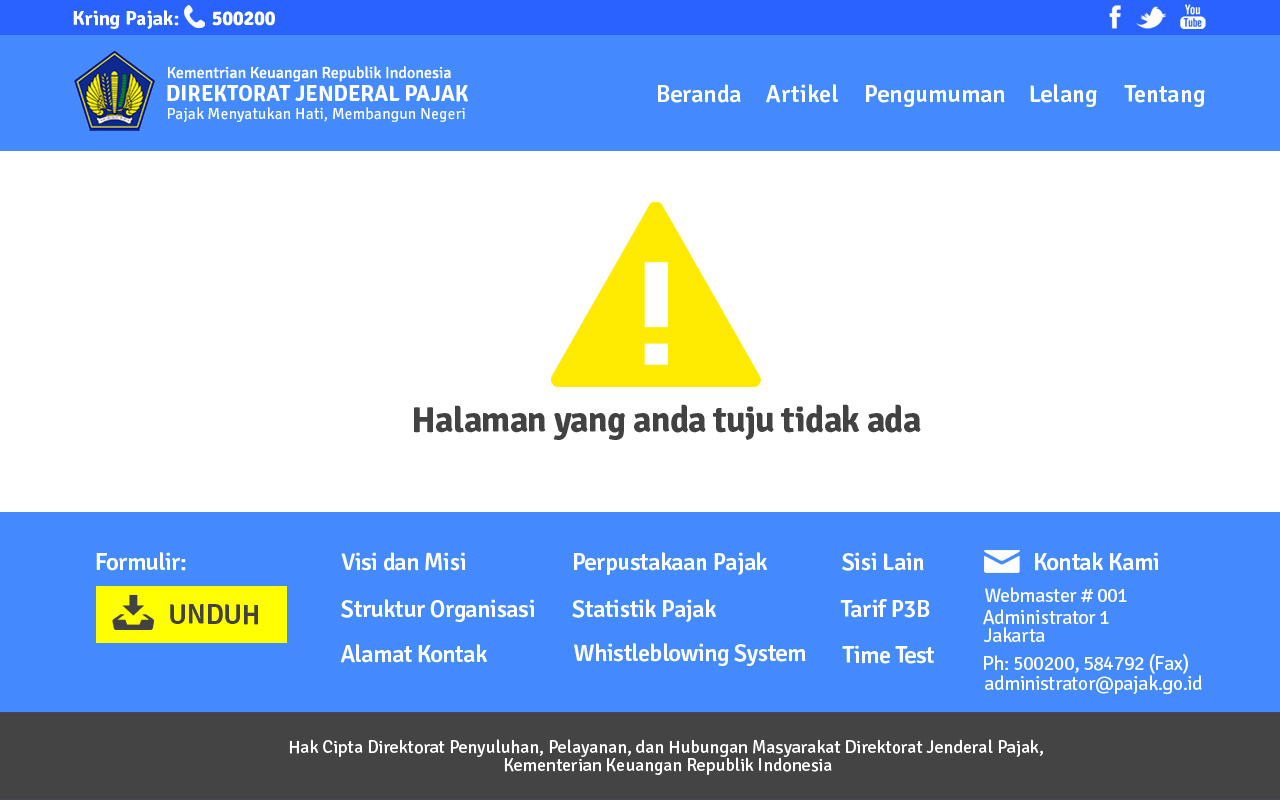
\includegraphics[width=\textwidth]
			{pics/error.jpg}
			\caption{\f{Clickable prototype} dari halaman akses yang \f{error}.}
			\label{fig:error}
		\end{figure}
	Selain pesan kesalahan, dibuat juga desain halaman \f{clickable prototype} yang menangani aksi pengguna yang melakukan tindakan keluar dari sistem yang bisa saja membuat kesalahan pada prosesnya. Gambar \ref{fig:peringatan} menunjukkan bahwa sistem memberitahu pengguna ketika pengguna akan menginggalkan \f{website} DJP setelah memilih salah satu dari aplikasi perpajakkan yang mengarah keluar \f{website}.
		\begin{figure}
			\centering
			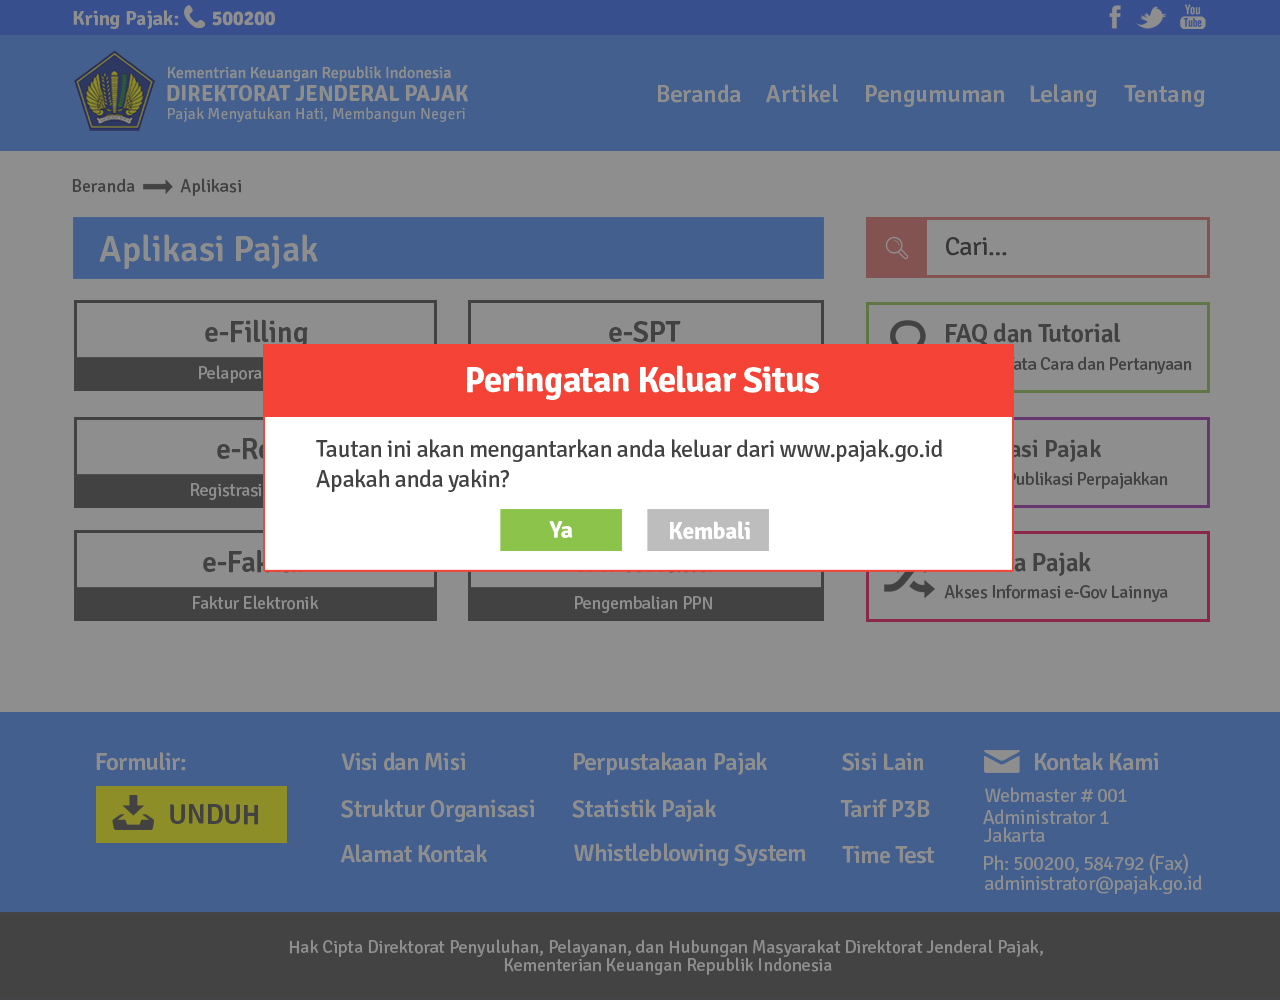
\includegraphics[width=\textwidth]
			{pics/peringatan.jpg}
			\caption{\f{Clickable prototype} dari halaman peringatan aksi pengguna.}
			\label{fig:peringatan}
		\end{figure}
	\item Halaman Layanan \\
	Halaman \f{clickable prototype} ini dibuat untuk memberikan informasi mengenai pelayanan yang disediakan oleh DJP Indonesia. Layanan dapat berupa informasi ataupun pengumuman peraturan. Gambar \ref{fig:layanan} menunjukkan fitur layanan untuk pencarian Kantor Pelayanan Pajak (KPP) terdekat yang dapat dicari pengguna.
		\begin{figure}
			\centering
			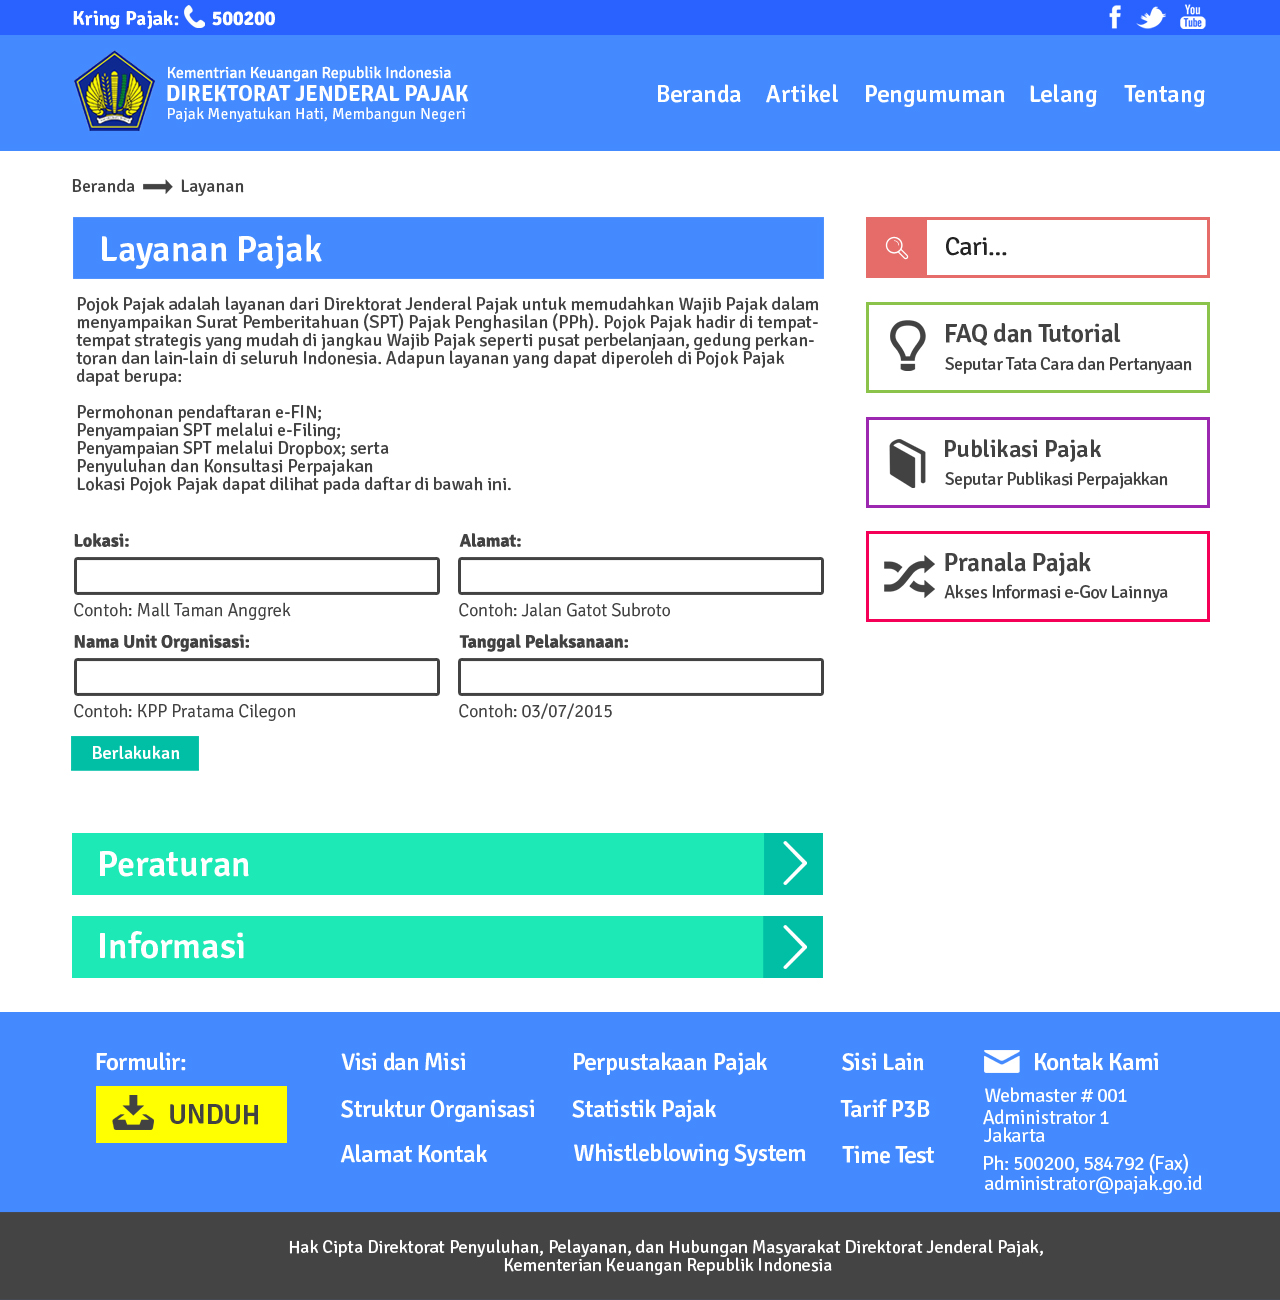
\includegraphics[width=\textwidth]
			{pics/layanan.jpg}
			\caption{\f{Clickable prototype} dari halaman layanan perpajakkan.}
			\label{fig:layanan}
		\end{figure}
	\item Halaman FAQ dan Tutorial \\
	Halaman ini dibuat untuk memperingkas dan memudahkan pencarian dokumentasi \f{website} bagi pengguna. Gambar \ref{fig:tutorial} menunjukkan halaman pertanyaan pengguna dan tutorial yang disatukan, hal tersebut bertujuan agar pengguna dapat mengakses semua informasi dalam tahap yang tidak panjang dan mudah.
		\begin{figure}
			\centering
			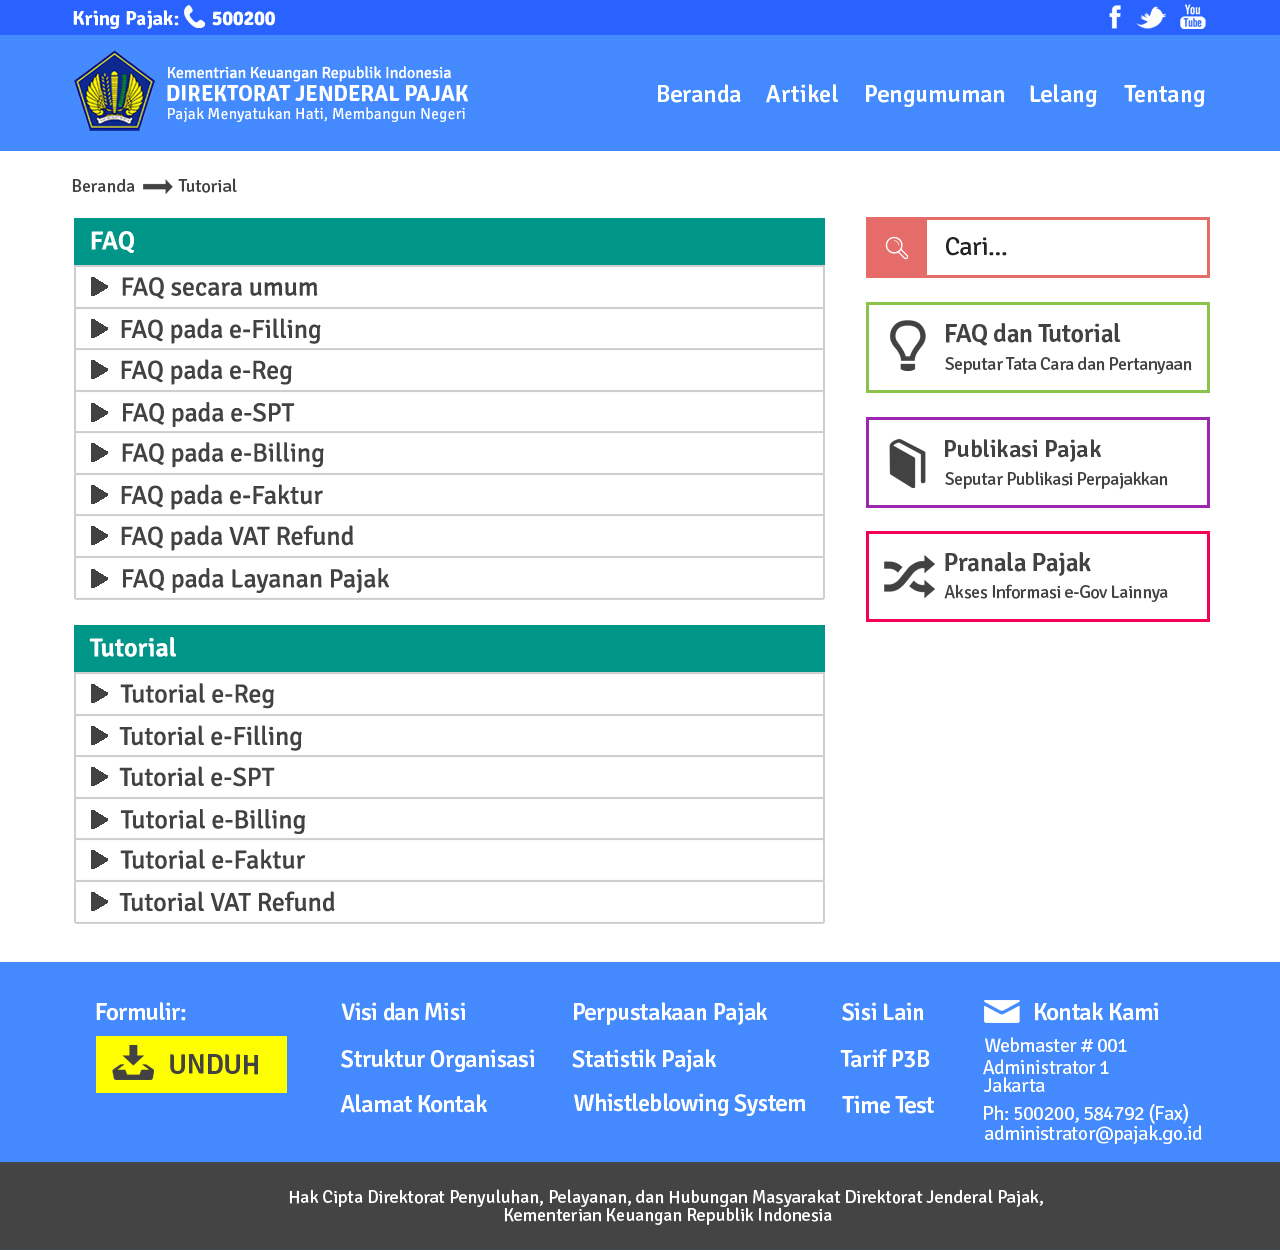
\includegraphics[width=\textwidth]
			{pics/tutorial.jpg}
			\caption{\f{Clickable prototype} dari halaman FAQ dan tutorial sebagai dokumentasi untuk pengguna.}
			\label{fig:tutorial}
		\end{figure}
	\item Halaman Login e-Filling \\
	Halaman \f{clickable prototype} untuk \f{login} ke aplikasi \f{e-Filling} dibuat dengan mendaur ulang tampilan sebelumnya. Gambar \ref{fig:login} tidak jauh berbeda dengan halaman \f{login} DJP Online sebelumnya, namun pada perubahan ini ditambahkan \f{captcha} yang berguna sebagai proteksi dan keamanan tambahan dari \f{website}.
		\begin{figure}
			\centering
			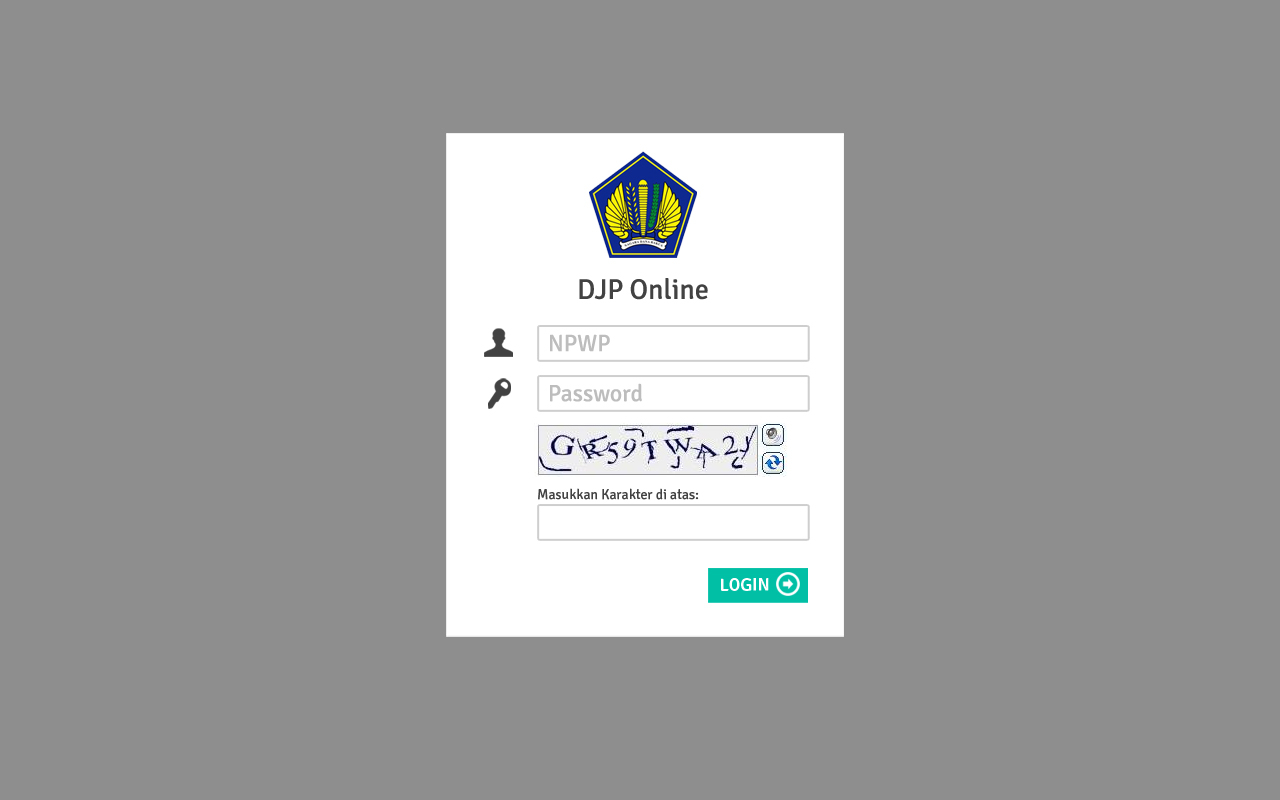
\includegraphics[width=\textwidth]
			{pics/login.jpg}
			\caption{\f{Clickable prototype} dari halaman login e-Filling.}
			\label{fig:login}
		\end{figure}
	\item Halaman Unduh \\
	Halaman \f{clickable prototype} untuk formulir dibuat secara berkelompok dan minimalis. Gambar \ref{fig:formulir} menunjukkan bahwa kesederhanaan halaman ditujukkan agar pengguna mudah untuk berinteraksi, sehingga terhindar dari kesalahan yang bisa saja terjadi.
		\begin{figure}
			\centering
			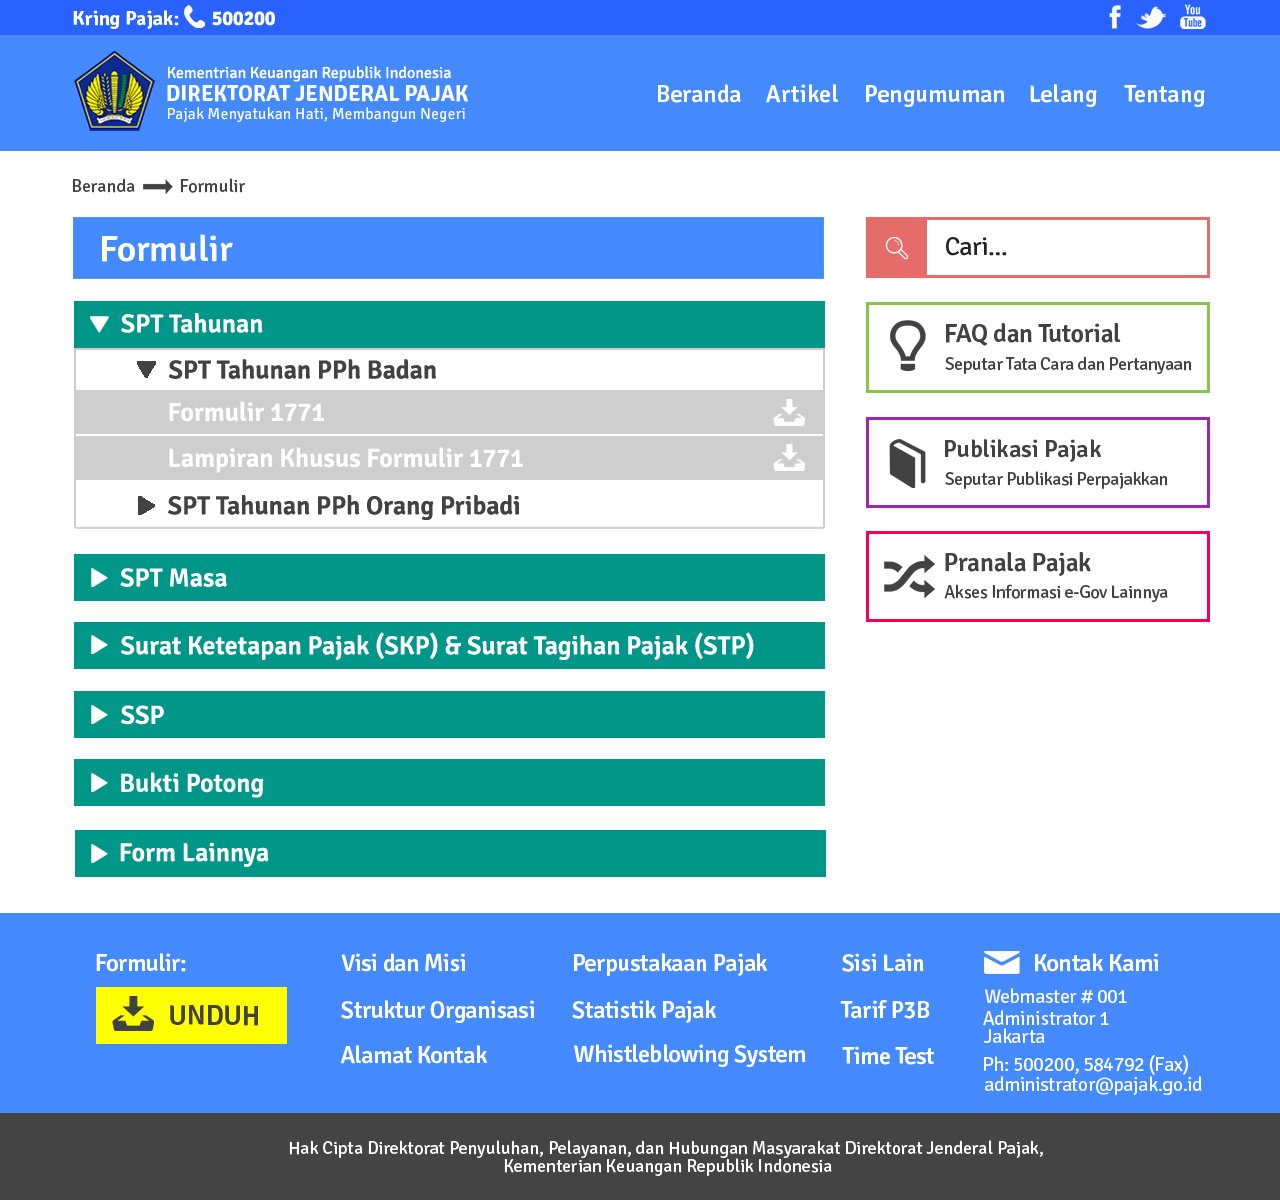
\includegraphics[width=\textwidth]
			{pics/formulir.jpg}
			\caption{\f{Clickable prototype} dari halaman unduh formulir.}
			\label{fig:formulir}
		\end{figure}
	\item Halaman Pranala \\
	Halaman ini berfungsi sebagai akses informasi antar \f{website e-government}. Gambar \ref{fig:pranala} menunjukkan bahwa halaman perbaikan \f{website} DJP ini dapat menampung dan bertukar informasi dengan \f{website} pemerintahan lainnya, sehingga pertukaran informasi dan juga data lebih mudah dilakukan.
		\begin{figure}
			\centering
			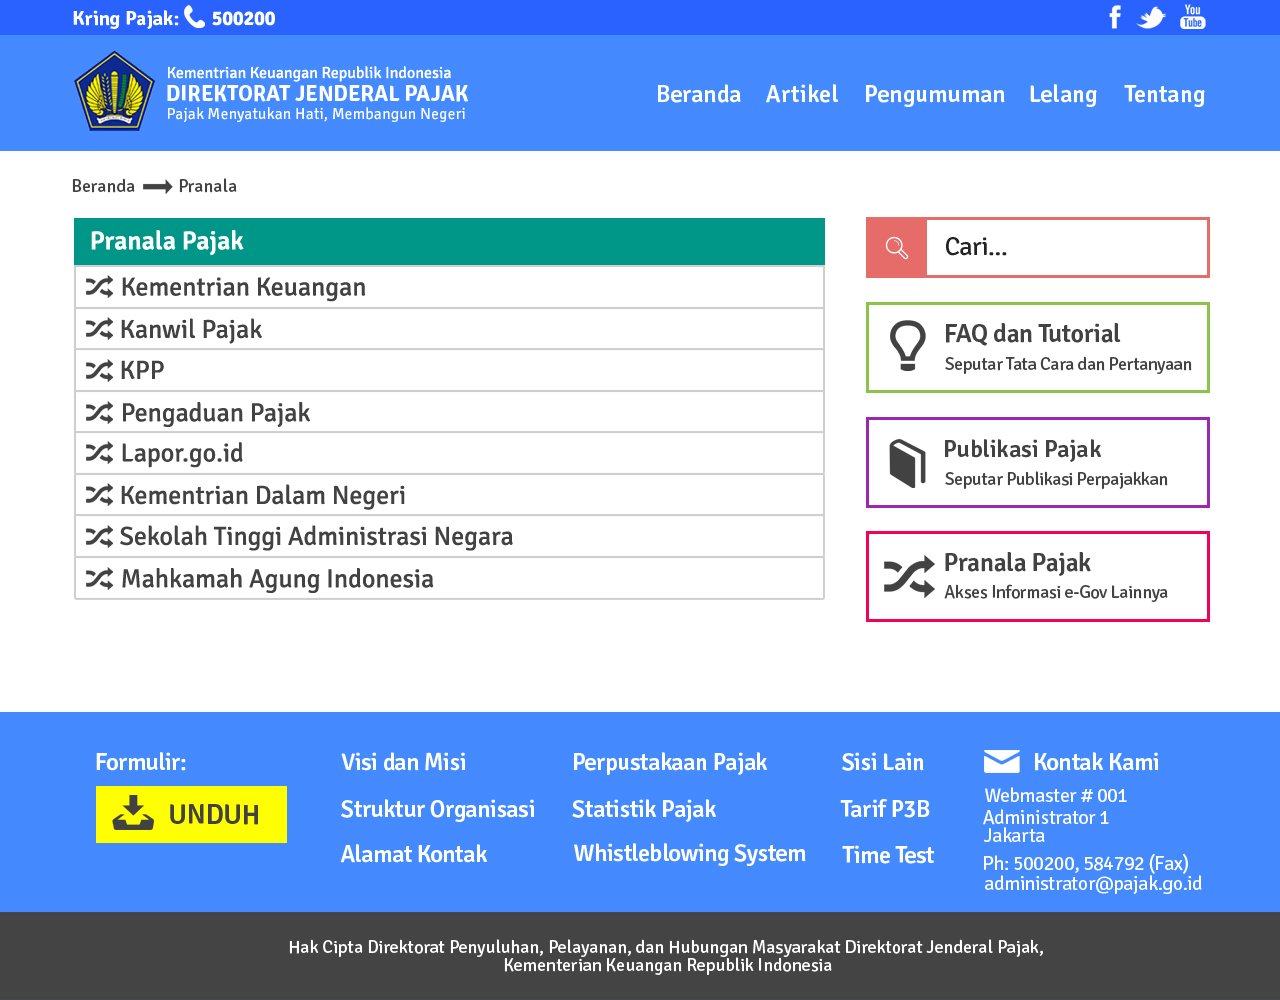
\includegraphics[width=\textwidth]
			{pics/pranala.jpg}
			\caption{\f{Clickable prototype} dari halaman pranala perpajakkan.}
			\label{fig:pranala}
		\end{figure}
\end{enumerate}
%-----------------------------------------------------------------------------%